\documentclass[10pt,a4paper]{article}
%\usepackage[ngerman]{babel}
\usepackage{color}
\usepackage{listings}
\usepackage{graphicx}
\usepackage{float}
%\usepackage{moreverb}
\usepackage[section]{placeins}
\usepackage{hyperref}

\setlength{\parindent}{0pt}

\title{\textbf{Shape Matching with Earth Mover's Distance}}
\author{Jon Volkmar\\
		Mart\'{i} Griera}
\date{}
\begin{document}

\maketitle

\section{Introduction}

\section{Experiment Setup}

\begin{figure}[ht!]
\centering
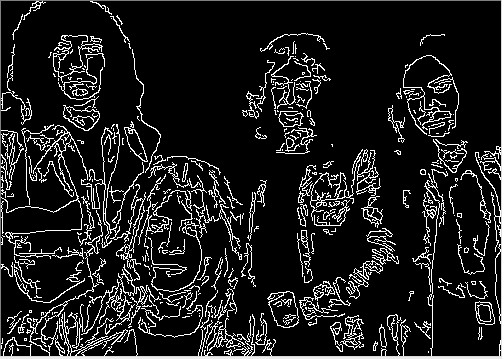
\includegraphics{canny_edge.png}
\caption{Output of Canny edge detector - edges are marked with a white outline}
\label{overflow}
\end{figure}

\begin{figure}[ht!]
\centering
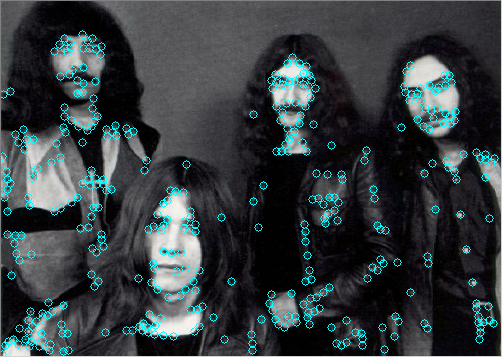
\includegraphics{harris_corner.png}
\caption{Harris Corner Detection - Detected corners are marked with blue circles}
\label{overflow}
\end{figure}

\begin{figure}[ht!]
\centering
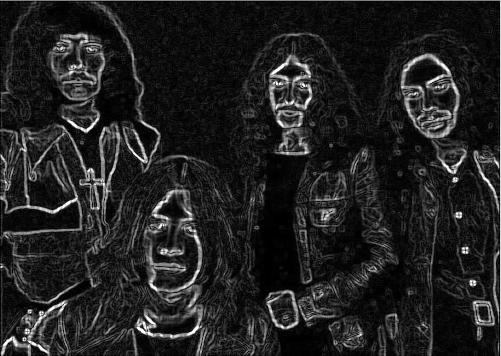
\includegraphics{sobel_intensity_gradient.png}
\caption{Image of the magnitude of the intensity gradient, calculated using the Sobel operator}
\label{overflow}
\end{figure}

\begin{figure}[ht!]
\centering
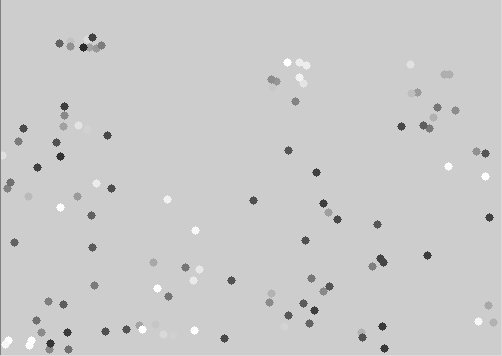
\includegraphics{weighted_point_set.png}
\caption{Each corner that is on a detected edge is given a weight, corresponding to the intensity gradient value at the same location, giving us a weighted point set. Low weights are black, high weights are white.}
\label{overflow}
\end{figure}

\section{Preliminary Results}

\begin{table}
    \caption{Queries on simple shape data set, 218 images \url{http://www.lems.brown.edu/vision/researchAreas/SIID/}}
    \begin{tabular}{|l|l|l|l|l|l|}
        \hline
        Query image & Match 1 & Match 2 & Match 3 & Match 4 & Match 5 \\ \hline

        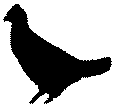
\includegraphics[width=20mm]{queries/bird09.png} &	
	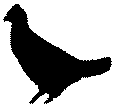
\includegraphics[width=20mm]{queries/bird09.png}  & 
	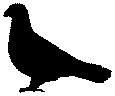
\includegraphics[width=20mm]{queries/bird18.png}  &
	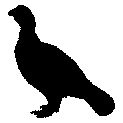
\includegraphics[width=20mm]{queries/bird07.png}  &
	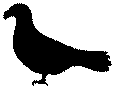
\includegraphics[width=20mm]{queries/bird19.png} &
	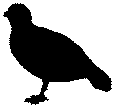
\includegraphics[width=20mm]{queries/bird02.png} \\ 
	~ & 0 & 6.51677 & 7.54387 &  7.87805 & 7.87867 \\ \hline

	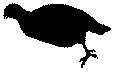
\includegraphics[width=20mm]{queries/bird04.png} &	
	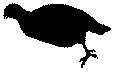
\includegraphics[width=20mm]{queries/bird04.png}  & 
	
\includegraphics[width=20mm]{queries/brick08.png}  &
	
\includegraphics[width=20mm]{queries/brick03.png}  &
	
\includegraphics[width=20mm]{queries/classic03.png} &
	
\includegraphics[width=20mm]{queries/brick04.png} \\ 
	~ & 0 & 6.53474 & 6.83729 & 6.87391 & 6.88357 \\ \hline

        \hline
    \end{tabular}
\end{table}


\begin{table}
    \caption{Queries on Buffy data set s5e6, 52 images \url{http://www.robots.ox.ac.uk/~vgg/data/buffy_pose_classes/t}}
    \begin{tabular}{|l|l|l|l|l|l|}
        \hline
        Query image & Match 1 & Match 2 & Match 3 & Match 4 & Match 5 \\ \hline

        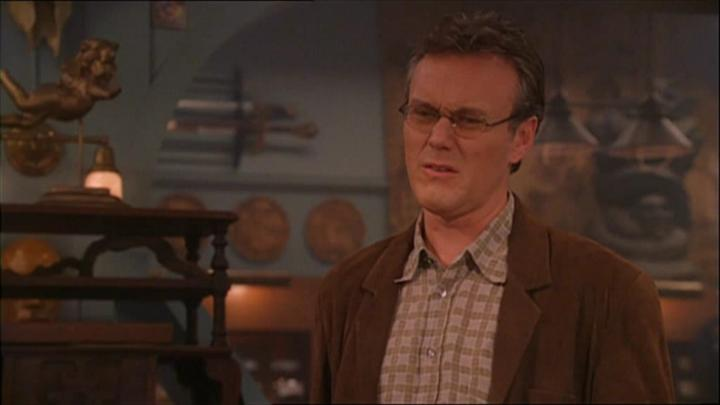
\includegraphics[width=20mm]{queries/015663.jpg} &	
	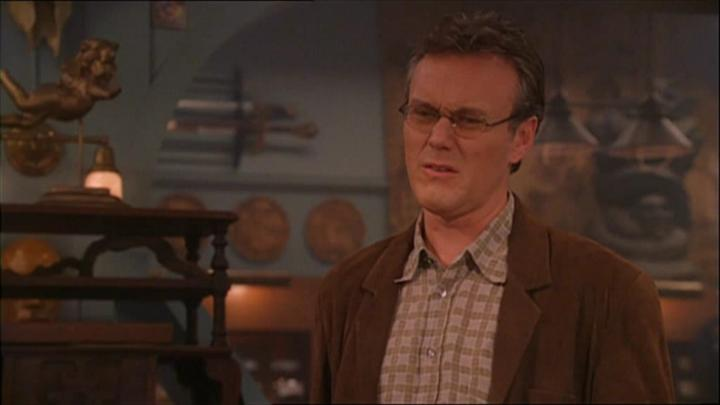
\includegraphics[width=20mm]{queries/015663.jpg} &	
	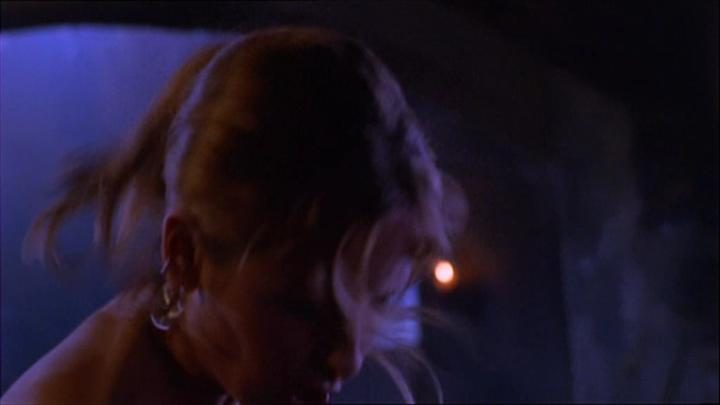
\includegraphics[width=20mm]{queries/019018.jpg}  &
	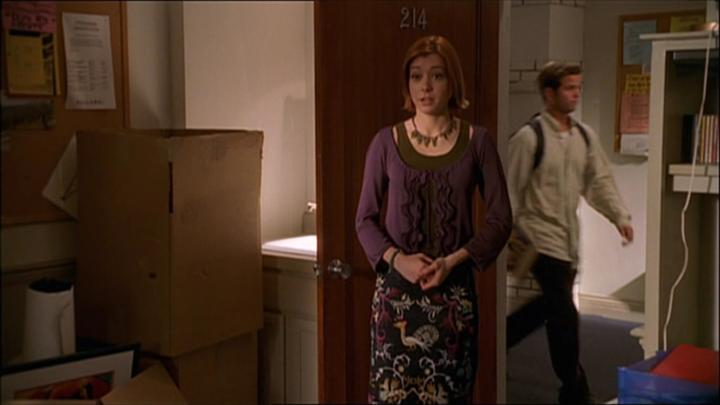
\includegraphics[width=20mm]{queries/012194.jpg}  &
	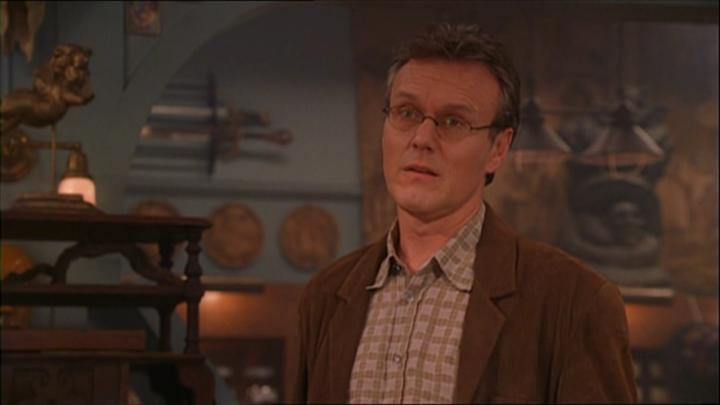
\includegraphics[width=20mm]{queries/015742.jpg} &
	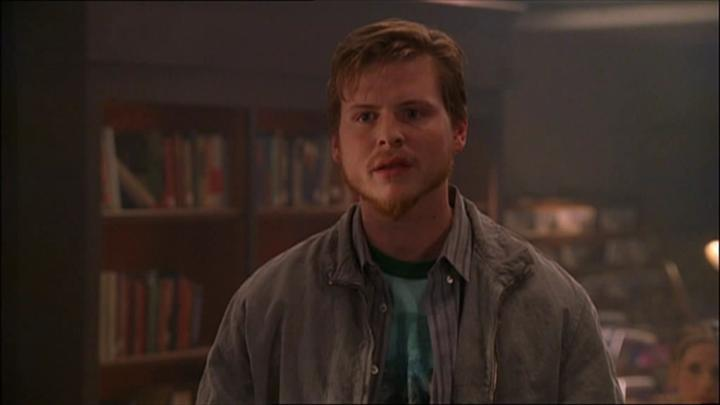
\includegraphics[width=20mm]{queries/022108.jpg} \\ 
	~ & 0 & 25.7924 & 34.351 &  37.4202 & 42.9105 \\ \hline

	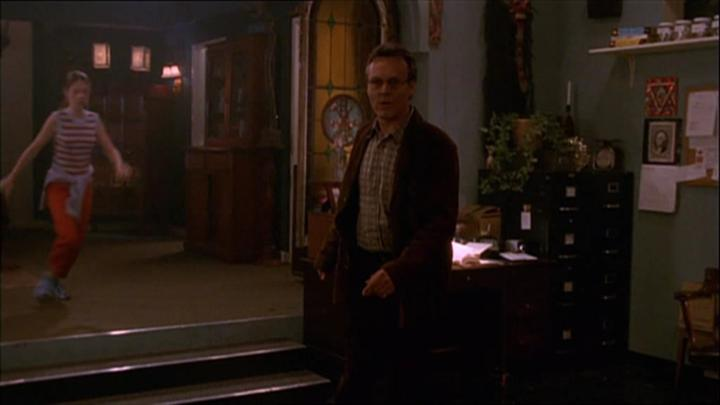
\includegraphics[width=20mm]{queries/046990.jpg} &	
	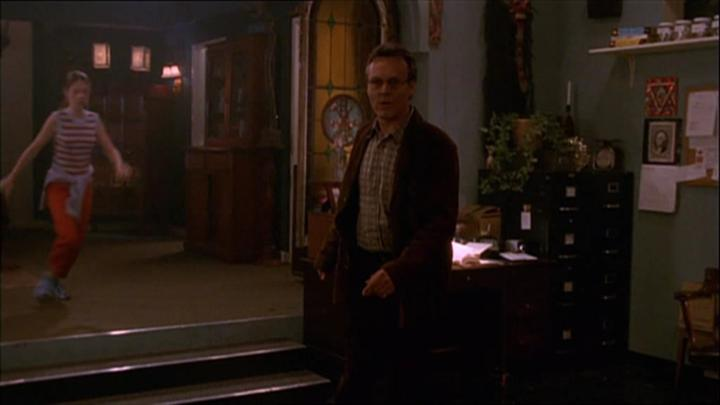
\includegraphics[width=20mm]{queries/046990.jpg}  & 
	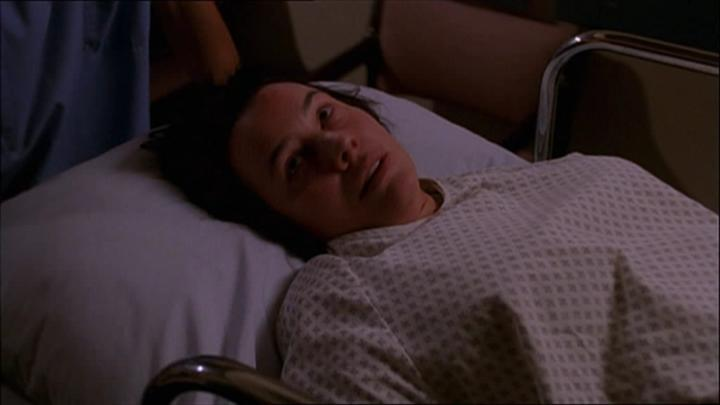
\includegraphics[width=20mm]{queries/012325.jpg}  &
	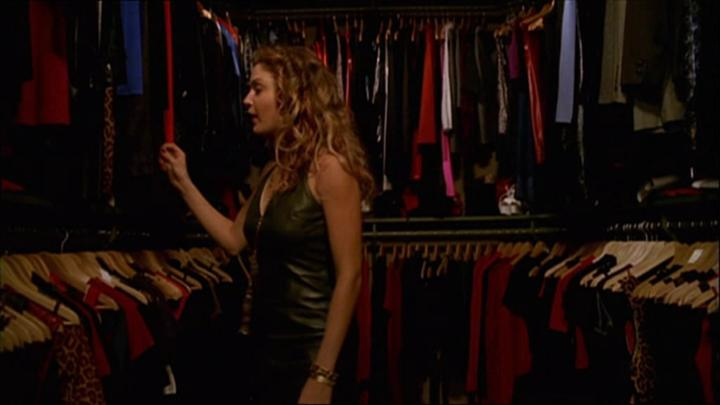
\includegraphics[width=20mm]{queries/032368.jpg}  &
	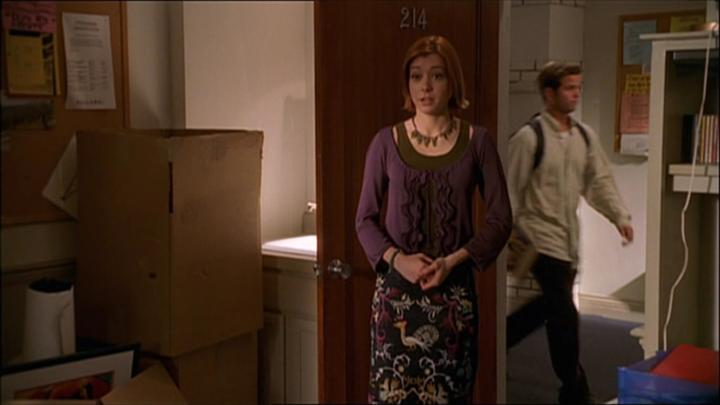
\includegraphics[width=20mm]{queries/012194.jpg} &
	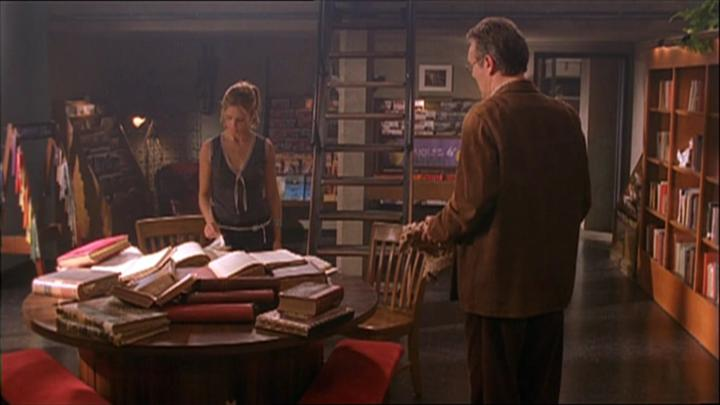
\includegraphics[width=20mm]{queries/015662.jpg} \\ 
	~ & 0 & 47 & 56.5078 & 56.8755 & 58.6826 \\ \hline

	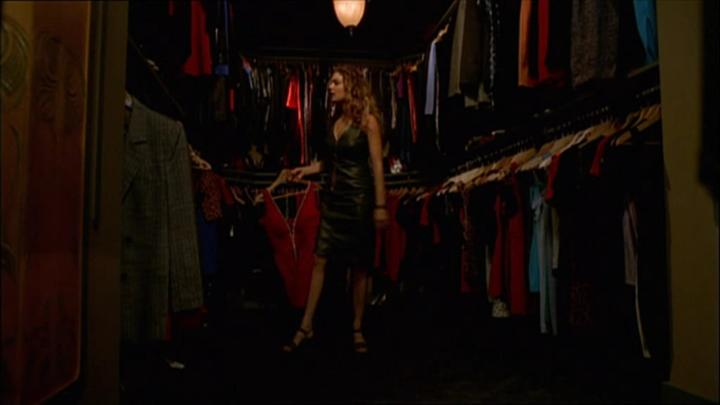
\includegraphics[width=20mm]{queries/032326.jpg} &	
	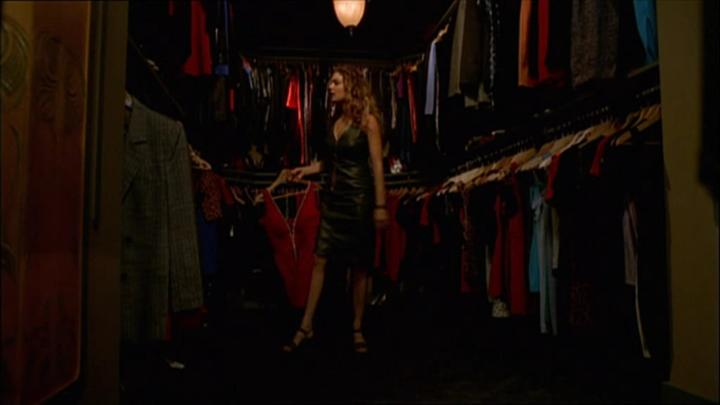
\includegraphics[width=20mm]{queries/032326.jpg}  & 
	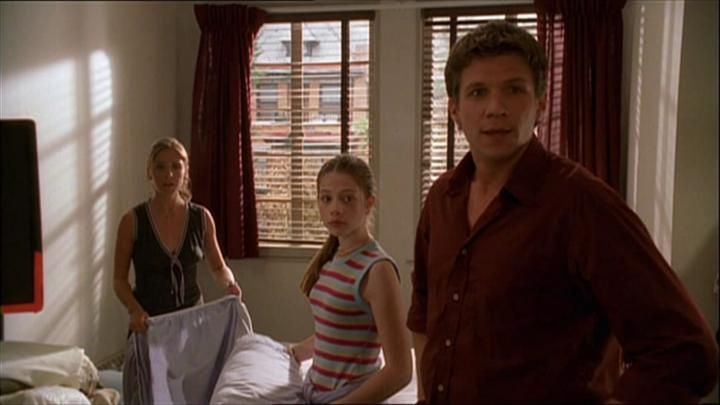
\includegraphics[width=20mm]{queries/012195.jpg}  &
	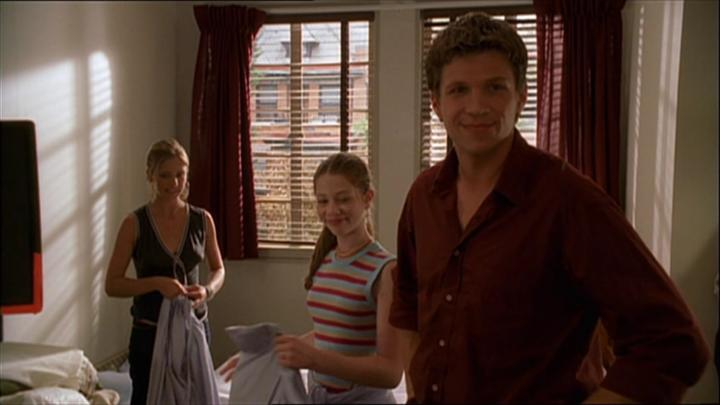
\includegraphics[width=20mm]{queries/012324.jpg}  &
	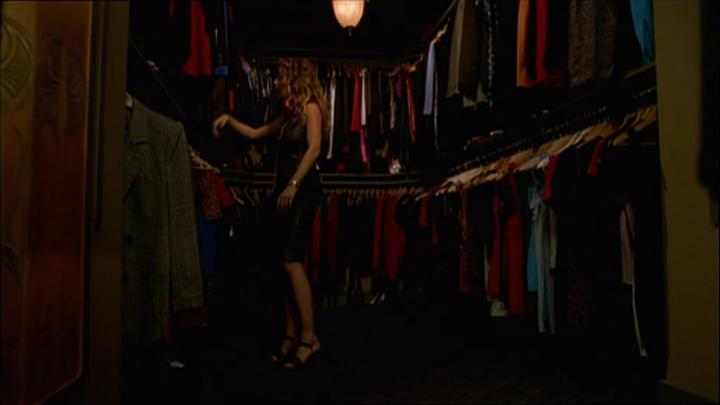
\includegraphics[width=20mm]{queries/032367.jpg} &
	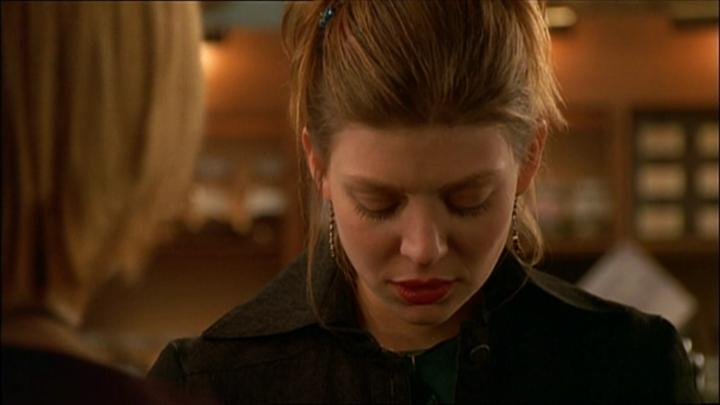
\includegraphics[width=20mm]{queries/052268.jpg} \\ 
	~ & 0 & 34.4968 & 35.6604 & 37.5272 & 42.8023 \\ \hline

        \hline
    \end{tabular}
\end{table}



\end{document}